%% LyX 2.3.6.1 created this file.  For more info, see http://www.lyx.org/.
%% Do not edit unless you really know what you are doing.
\documentclass[twocolumn,conference]{IEEEtran}
\usepackage[T1]{fontenc}
\usepackage[latin9]{inputenc}
\usepackage{array}
\usepackage{booktabs}
\usepackage{multirow}
\usepackage{amsmath}
\usepackage{graphicx}
\usepackage[unicode=true,
 bookmarks=true,bookmarksnumbered=true,bookmarksopen=true,bookmarksopenlevel=1,
 breaklinks=false,pdfborder={0 0 1},backref=false,colorlinks=false]
 {hyperref}
\hypersetup{pdftitle={Small-Dictionary LCA Sparse Coding for Low-Power Pattern Recognition in Edge Devices},
 pdfauthor={Lawrence Roman Quizon},
 pdfborderstyle=,pdfpagelayout=OneColumn,pdfnewwindow=true,pdfstartview=XYZ,plainpages=false}

\makeatletter

%%%%%%%%%%%%%%%%%%%%%%%%%%%%%% LyX specific LaTeX commands.
%% Because html converters don't know tabularnewline
\providecommand{\tabularnewline}{\\}

%%%%%%%%%%%%%%%%%%%%%%%%%%%%%% User specified LaTeX commands.
% for subfigures/subtables

\usepackage[caption=false,font=footnotesize]{subfig}
\usepackage{graphicx}

\let\oldincludegraphics\includegraphics
\renewcommand\includegraphics[2][]{%
  \oldincludegraphics[width=\linewidth]{#2}
}

\makeatother

\begin{document}
\title{Small-Dictionary LCA Sparse Coding for Low-Power Pattern Recognition
in Edge Devices}
\author{\IEEEauthorblockN{Lawrence~Roman~A.~Quizon, Marc D. Rosales, Anastacia B. Alvarez}\IEEEauthorblockA{Electrical and Electronics Engineering Institute\\
 University of the Philippines-Diliman\\
 Quezon City, Philippines}}
\maketitle
\begin{abstract}
Sparse coding can be used to perform feature extraction and classification
on high-dimensional data and is a mechanism which biological neural
sensory systems employ. The Locally Competitive Algorithm (LCA) is
a sparse coding mechanism compatible with the memristor crossbars
used for in-memory computing, and is shown here to have promise of
being effective with low enough power and scale to be suitable for
use in edge devices for classifying/compressing signals such as energy
harvesting contexts and images on the edge. This paper explores the
tradeoffs of different aspects of the algorithm such as the dictionary
completeness, activation threshold, and number of iterations in order
to increase LCA efficiency in memristor crossbars on the edge in anticipation
of challenges such as the quantization, variance and energy constraints.
A 100\% accuracy was achieved for classifying 5 different gestures
from synthetic solar energy harvesting data using only 2 iterations
of the LCA on a very small 50-element dictionary.
\end{abstract}


\IEEEpeerreviewmaketitle{}

\section{Introduction}

In the increasingly more popular paradigm of edge computing, information
processing takes place not only in powerful servers in \textquotedbl center
nodes\textquotedbl{} but also in the \textquotedbl edges\textquotedbl{}
of a network. This allows networks of IoT devices like wireless sensors
designed for low-power operation tasks to save even more energy by
avoiding energy expensive transmission over multiple hops or long
distances. Because of their heavy use of the multiply-and-accumulate
(MAC) operation, most signal processing algorithms have trouble being
implemented on the edge. Using novel memristor devices connected in
a crossbar architecture is a big leap towards the energy-efficient
implementation of the MAC-operation on the edge \cite{sebastian2020memory}.

Sparse coding is one such algorithm that has been successful for a
variety of applications such as face recognition \cite{wright2009sparse}
and visual tracking \cite{zhang2013sparse} and has now also found
use in energy harvesting context sensing \cite{xu2018keh}. While
there are a variety of algorithms that exist to obtain sparse representations,
an algorithm based on competing neurons, the ``locally competitive
algorithm'' (LCA) is particularly promising for use in edge computing
due to its compatibility with the memristor crossbar architecture,
on which it has been implemented before \cite{sheridan2017sparse}.
In contrast with popular neural networks that do MAC operations with
many weight matrices for each neuron on the previous layer, sparse
coding in LCA has the potential to be effective with a single crossbar
for the dictionary, reducing concerns about memristor variation and
scaling problems.

In this paper, accuracy-energy/size tradeoffs with LCA sparse coding
parameter selection, choices of dictionary sizing, and number of quantization
levels were explored in anticipation of challenges in the crossbar
implementation stemming from quantization, memristor variation and
energy constraints.

To evaluate the tradeoffs, sparse coding is used to classify 5 different
gestures inferred from the energy harvesting response of a solar cell,
synthesized using SolarGest \cite{ma2019solargest} with the parameters
outlined in Table \ref{solargest parameters}. In this paper, the
current waveforms generated were subsampled into feature vectors of
length $128$. In the end, this paper produced an LCA sparse coding
scheme able to classify 5 different gestures from the current waveform
of the solar cell above which these gestures are made to 100\% accuracy
with only 2 LCA iterations in a $128\times50$ dictionary matrix.

\section{Classification using LCA}

Sparse coding attempts to represent an arbitrary vector $x$ by representing
it as a linear combination of a set of basis functions $D$, called
the dictionary. The choice of basis functions can vary. They can be
obtained from standard bases, can be completely random, or made/learned
from training feature vectors. The objective of sparse coding is to
represent $x$ in terms a vector of coefficients $a$ (called the
sparse representation) such that $x=Da^{T}$, but with the constraint
that $a$ be sparse. This can be formulated as the following:
\begin{equation}
min_{a}(|x-Da^{T}|_{2}+\lambda|a|_{0})\label{eq:1}
\end{equation}

where $|\cdot|_{2}$ and $|\cdot|_{0}$ are the $L^{2}$ and $L^{0}$
norms, terms which prioritize reconstruction accuracy and sparseness
respectively. This optimization problem is non-convex and NP-hard.
The LCA is a biologically inspired algorithm for approximating the
solution $a$ \cite{rozell2008sparse}. In the LCA, dictionary elements
are modelled as leaky neurons with membrane potentials. The membrane
potential $u$ of an LCA neuron can be described by the difference
equation \cite{sheridan2017sparse}:
\begin{equation}
u_{n+1}=\frac{1}{\tau}(-u_{n}+(x-Du_{n}^{T})^{T}D+a_{n})\label{eq:2}
\end{equation}
\[
a_{n}=\begin{cases}
u_{n} & ifu>\lambda\\
0 & otherwise
\end{cases}
\]

Governed by the parameters $\tau$ and $\lambda$, the change in the
potential $u$ is proportional by $1/\tau$ to three terms: its size
$(-u)$, its similarity to the input $(x^{T}D)$ and inhibition from
similar neurons $(a(D^{T}D-I_{n}))$ where $D^{T}D-I_{n}$ is the
neuron similarity matrix. If a neuron's potential $u$ is above the
threshold $\lambda,$ it is deemed active, and it starts contributing
to the inhibition term. We use the hard thresholding function for
the thresholding in this paper for simplicity. The compatibility of
the LCA with memristor crossbars stems from the fact that in this
algorithm, the only matrix that is being used is D and only with matrix-vector
multiplications.

Compression using sparse coding is simple, since the values and indexes
of the nonzero sparse coefficients can simply be taken as the compressed
signal. Classification can be done using sparse coding by appending
multiple dictionaries learned for different classes together. After
learning each class dictionary $D_{i}$ for class $i$, the global
dictionary is then made by concatenating the class dictionaries $D=[D_{1},D_{2},...,D_{N}]$
for $N$ classes. The usual method to infer the class of $x$ from
$a$ is called minimal subspace search (MSS). In MSS, given the sparse
representation $a$ from the global dictionary, the signal is reconstructed
using only coefficients associated with each class dictionary- and
the predicted class is that of the class dictionary that produces
the minimum reconstruction error (residue). Getting the residue for
MSS is too computationally expensive to do on edge devices, even with
the help of memristor crossbars, and hence we opt to just take the
class of the largest sparse coefficient $argmax(a)$. Good classification
accuracies are obtained despite this, and so it is shown that this
scheme can be enough for the gesture classification done in this paper-
indicating possible viablity for other EH sensing applications as
well.

\begin{table}
\centering{}\caption{SolarGest Input Parameters with Hand Size Statistics taken from Chia
et al. \label{solargest parameters}\cite{chia2020anthropometric}}
\begin{tabular}{ccc}
\toprule 
Parameter & Mean & StDev\tabularnewline
\midrule
\midrule 
Hand Diameter & $9.72cm$ & $1.14cm$\tabularnewline
\midrule 
Hand Pos Low & $2cm$ & $0.1cm$\tabularnewline
\midrule 
Hand Pos High & $10cm$ & $1cm$\tabularnewline
\midrule 
Gesture Speed & $20cm/s$ & $1cm/s$\tabularnewline
\midrule 
Hand Height (for horizontal gestures) & $5cm$ & $1cm$\tabularnewline
\midrule 
Solar Cell Radius & $2cm$ & \tabularnewline
\midrule 
Light Intensity & $200lux$ & \tabularnewline
\midrule 
Solar Cell Current Density & $7mA/cm^{2}$ & \tabularnewline
\bottomrule
\end{tabular}
\end{table}

A total of 3000 current waveforms were generated using SolarGest containing
5 gestures, 500 of which were used as the training set and the rest
were used as the test set. The class dictionaries $D_{i}$ were learned
using basis pursuit denoising (BPDN) in the SPORCO software \cite{wohlberg2017sporco}.
The global dictionaries hence had a total of $K*Nclasses$ bases,
where $N$ is the number of classes and $K$ is the number of bases
in a class dictionary. A total of 4 global dictionaries with $K=150,50,25,10$
were used, along with an unlearned dictionary containing the test
vectors and a completely random dictionary. 

\section{Results}

\begin{figure}
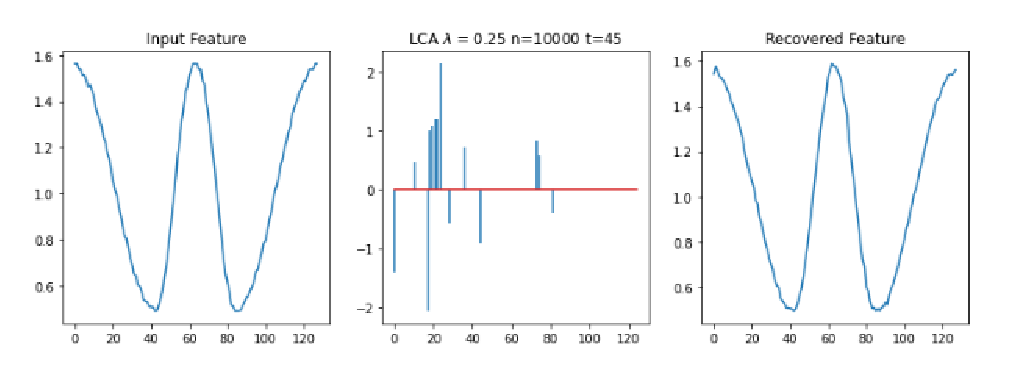
\includegraphics{pasted24}\caption{Sample Gesture Sparse Coding using $K=25,Q=\infty$ Dictionary. \label{sample sparse code}}
\end{figure}


\subsection{Compressive Sensing}

In compressive sensing, the results show that a dictionary as overcomplete
as possible is better for the same number of operations and generally
for any number of quantization levels.

Shown in Figure \ref{reconerror} is a sample feature reconstruction
of various gestures. The LCA fails to converge (it can diverge in
discrete time, despite stability in continuous time) to a solution
using either the untrained dictionary containing only the training
feature vectors or the random dictionary for the parameters shown.
For the trained dictionaries, the LCA can settle into a good sparse
representation for all $K=10,25,50,150$ where $K$ is the number
of dictionary elements per class (albeit with a bit of difficulty
with the $K=150$ dictionary).

Dictionaries with less elements generally lead to more reconstruction
error for the same number of iterations, as shown in Figure \ref{reconerror}
(a). However, introducing too many elements will introduce a lot of
unnecessary neurons to the code whose feature space (the loose set
of feature vectors that will activate it strongly) will overlap with
each other, introducing oscillatory behavior in the LCA and generally
poorer reconstruction. While overcomplete dictionaries should theoretically
allow better sparse reconstructions, the dynamics of the LCA system
in discrete time introduces mistakes in single iterations that are
more significant the more competition there is (more similar receptive
fields between the LCA neurons). 

\begin{figure}
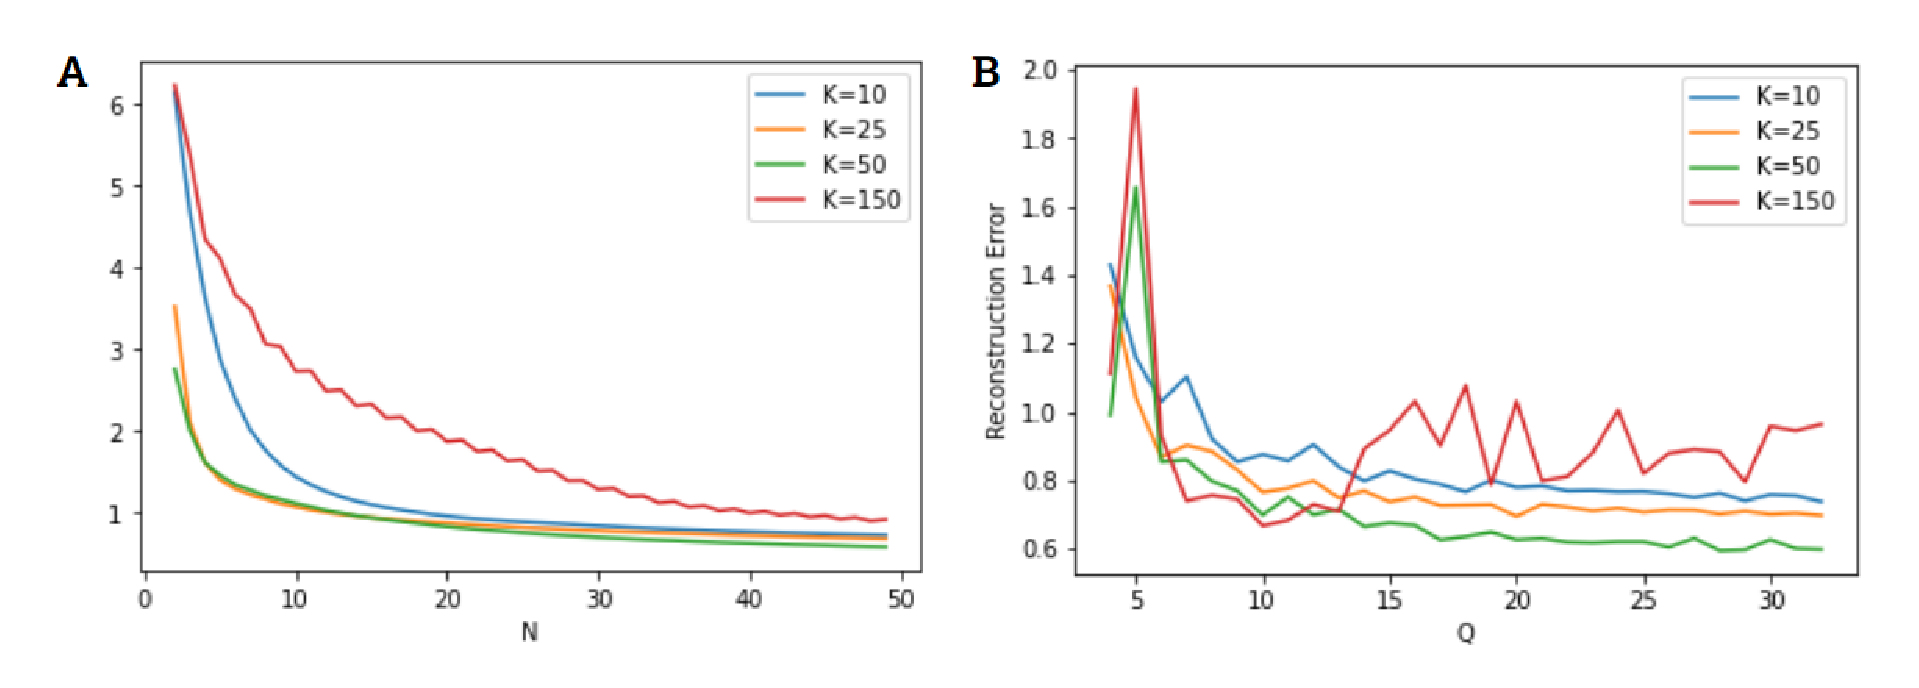
\includegraphics{pasted26}\caption{Average reconstruction error $|x-Da|_{2}$ (a) for each dictionary
vs $n$ ($Q=\infty)$. $\lambda,\tau=0.25,40$. (a) vs number of quantization
levels $Q$ vs $K$ at $n=45$. $\lambda,\tau=0.25,40$. \label{reconerror}}
\end{figure}
 

When the dictionaries are quantized, the lower the quantization number
the lower the reconstruction accuracy gets for a specific number of
iterations. This reconstruction accuracy does not get better over
more iterations, resulting in a sort of steady-state error, as seen
in Figure \ref{reconerror} (b). The quantization can sometimes randomly
be better for the reconstruction, and $K=150$ having more elements
is subject to this effect the most while the others can be observed
to get less random fluctionations as the dictionaries get smaller. 

\subsection{Pattern Recognition}

Using as few iterations for the LCA as possible is ideal to lower
the energy consumption of the computation in a memristor crossbar.
From equation \ref{eq:2}, each iteration of the LCA only needs two
vectors to be multiplied to the dictionary $D,$ and hence, the number
of crossbar operations is twice the number of iterations $c=2n$.
Furthermore, a dictionary as small as possible is also ideal for a
smaller crossbar, which also directly reduces the energy consumption
of the computation.

Lower $K$ and $Q$ result in better classification accuracies suggesting
that concatenating dictionaries as undercomplete (as low $K)$ as
possible for each class is ideal for classification using LCA. It
may be that by reducing the number of dictionary elements, the learned
elements are forced to be more orthogonal to each other, increasing
the discriminative ability at the cost of reconstruction accuracy
(for which overcomplete dictionaries are better, since infinite sparse
solutions exist) as was found in the previous section.

Optimal combinations for $\tau$ and $\lambda$ can be seen in the
grid sweeps in Figure \ref{fig:-colormaps-of}. While for some dictionaries
the classification accuracies are already too high (lots of $\tau-\lambda$
lead to 100\% accuracy), optimal combinations of $\tau-\lambda$ as
a function of $n$ and $Q$ exist for the other dictionaries. The
derivation of analytical expressions for guidelines of optimal combinations
from this empirical data is possible, the derivation of which may
be good for more difficult classification tasks.

These maps are non-concave, since many local maxima can be found through
the grid search. Thus, the use of gradient ascent and the like will
be subject to many local maxima, and not be guaranteed to reach the
optimal parameters. Despite that, stochastic gradient ascent still
tends to reach a set of parameters that give near-optimal accuracy
for any $n,K,Q$ combinations, given good guesses for the starting
points which tend to be $\tau\in(20,30),\lambda\in(0.1,0.3)$.
\begin{table}
\centering{}\caption{Maximum Accuracies found for grid search in Figure \ref{fig:-colormaps-of}\label{maximums}}
\begin{tabular}{cccc}
\toprule 
Dictionary & N & $\lambda,\tau$ & Accuracy\tabularnewline
\midrule
\midrule 
\multirow{2}{*}{$K=150$} & 2 & $(0.234,25.873)$ & $0.67$\tabularnewline
\cmidrule{2-4} \cmidrule{3-4} \cmidrule{4-4} 
 & 5 & $(0.217,12.381)$ & $0.666$\tabularnewline
\midrule 
\multirow{2}{*}{$K=50$} & 2 & $(0.222,23.492)$ & $0.73$\tabularnewline
\cmidrule{2-4} \cmidrule{3-4} \cmidrule{4-4} 
 & 5 & $(0.094,25.079)$ & $0.772$\tabularnewline
\midrule 
\multirow{2}{*}{$K=25$} & 2 & $(0.117,29.841)$ among many & $1$\tabularnewline
\cmidrule{2-4} \cmidrule{3-4} \cmidrule{4-4} 
 & 5 & $(0.050,21.111)$ among many & 1\tabularnewline
\midrule 
\multirow{2}{*}{$K=10$} & 2 & $(0.122,51.270)$ among many & 1\tabularnewline
\cmidrule{2-4} \cmidrule{3-4} \cmidrule{4-4} 
 & 5 & $(0.261,59.206)$ among many & 1\tabularnewline
\bottomrule
\end{tabular}
\end{table}

\begin{figure}
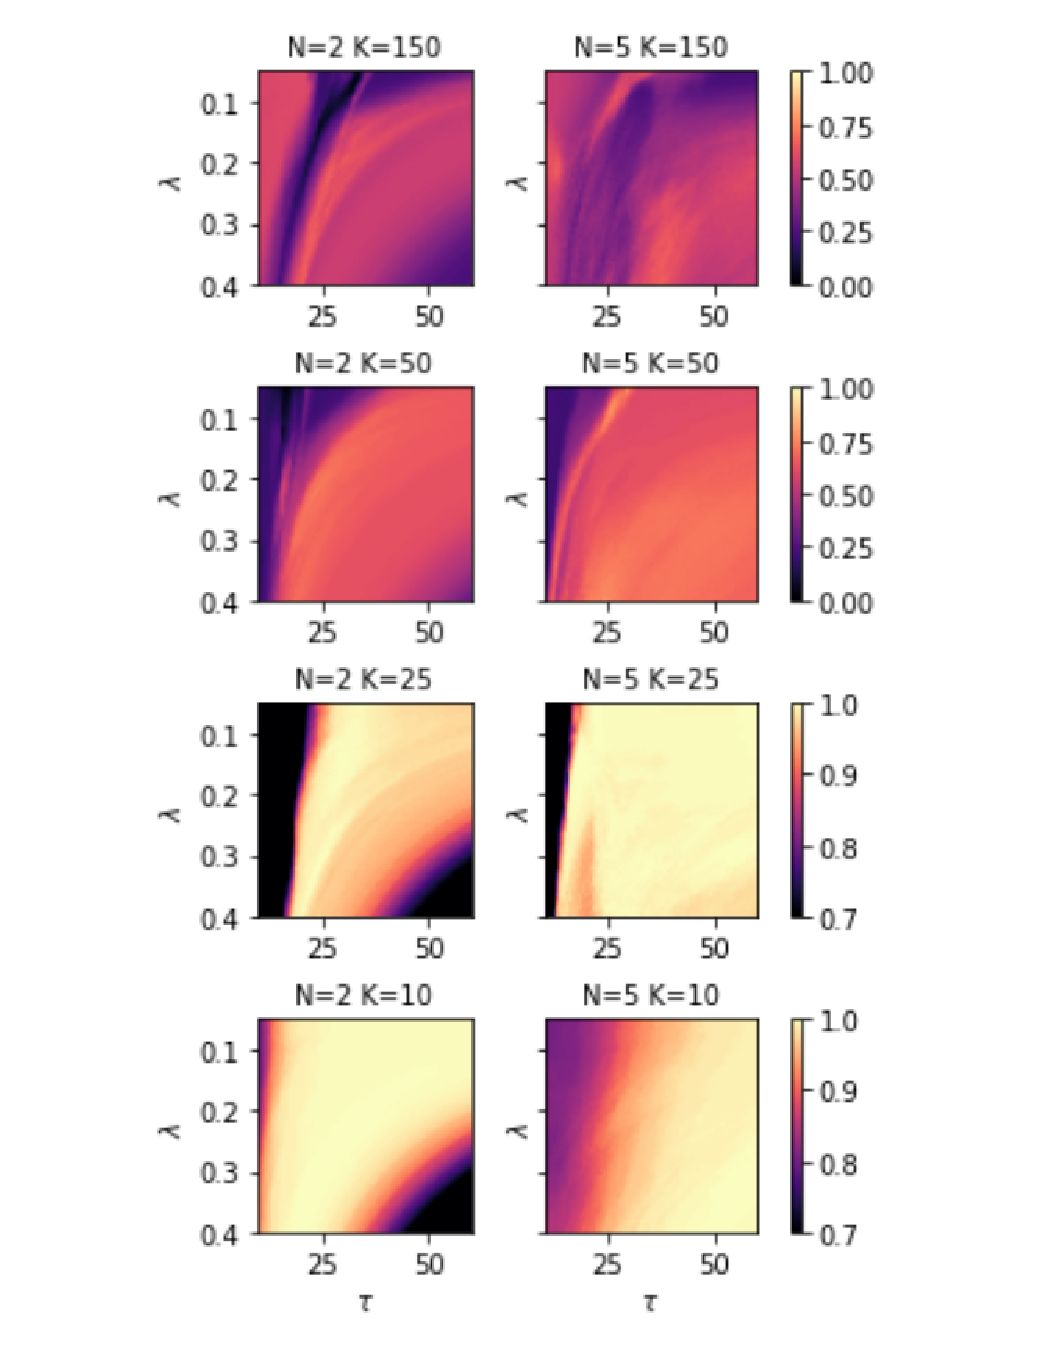
\includegraphics{pasted35}\caption{$\tau-\lambda$ grid search map of classification accuracies at $Q=10$.\label{fig:-colormaps-of}}
\end{figure}

In general, lower $K$ dictionaries perform better against less quantization
levels. However, it can be seen from Figure \ref{acc for diff q n=00003D2}
that, holding$K$ constant, less quantization levels can be better
for the classification accuracy. In particular, it can be noted that
$K=10$ and $25$ plummet after $Q=10$ and $9$ respectively. After
$Q=8,$ all the dictionaries work suboptimally. This may be a somewhat
random contribution where some quantizations are coincidentally better.

\begin{figure}
\includegraphics{pasted30}\caption{Line graph of classification accuracies for $K=150,50,25,10$ at differing
$Q$, $n=2$. Note how there is a specific $Q$ for some $K$ at which
the accuracy starts plummeting. Gradient Ascent was used to obtain
these.\label{acc for diff q n=00003D2}}
\end{figure}

The high $K$ dictionaries also benefit from more iterations as seen
in Figure \ref{acc vs n}, while the lower $K$ dictionaries actually
suffer with higher $n$, worse in the middle ranges. This can likely
be due to the fact that a high $K$ allows for more coincidentally
activated elements of the wrong class, while more quantized (lower
$Q$) dictionaries are more susceptible to a sort of steady state
error as the number of iterations increase. 

$K=150$ performing better for odd iterations may be due to oscillation
in the LCA output, where the input $x$ tends to activate a specific
set of neurons $a_{x}\subset a$, but these neurons are extremely
similar to each other and thus tend to beat each other down through
inhibition in the very next cycle. This is removed by decreasing $K,$
since forcing the BPDN dictionary learning algorithm to work with
less elements forces it to make the elements more dissimilar.

\begin{figure}
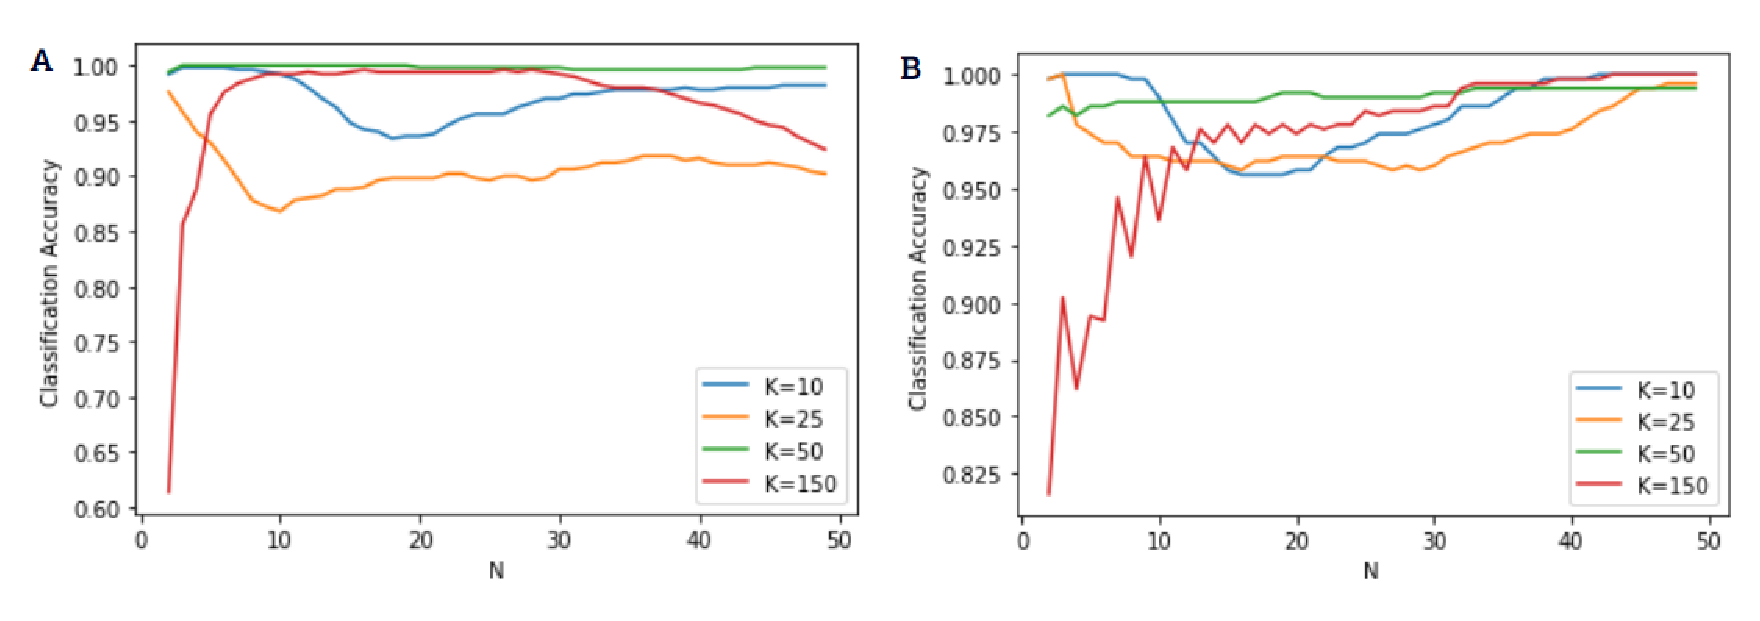
\includegraphics{pasted25}\caption{Line graph of classification accuracy vs number of iterations for
$Q=16$ (a) and $Q=\infty$ (b) \label{acc vs n}}
\end{figure}


\subsection{Effects of Conductance Variation on Pattern Recognition}

The standard deviation $\sigma$ of the conductance of a memristor
crossbar is around the difference of two conductance levels in Sheridan
et al. \cite{sheridan2017sparse}, and so that is used as the reference
for the conductance variation, henceforth noted as $\Delta L_{Q}$.
Shown in Figure \ref{hist} are the histograms of each dictionary
on the lowest quantization level $Q$ where they achieve great accuracy
results, since a low $Q$ is ideal for memristor fabrication and write
methods.

Standard deviations as much as $\Delta L_{Q}$ can render the scheme
unusable, and it is visible that even a $0.1\Delta L_{Q}$ variation
can affect the accuracy to as low as $80\%$, which needs to be noted
when choosing the memristor to implement the scheme with. Fortunately,
the scheme is shown to work to very low $Q$, which may let fabricators
optimize the memristors for less variation.

Visually, $K=10$ gives the best distribution, with the highest number
of still-100\% accuracies at $0.1\Delta L_{Q}$, while having waveforms
similar to $K=50$ and $25$ in the other standard deviations. While
$K=150$ is showing terrible results here, that is because it is being
run at $Q=12,$ since its best accuracies can only be obtained at
$n$ higher than 2 (as seen in Figure \ref{acc vs n}).

\begin{figure}
\includegraphics{pasted37}\caption{Histograms of each dictionary on the lowest quantization level $Q$
where they achieve great accuracy results as seen in Figure 7 for
$n=2$. $K,Q=(150,12),(50,8),(25,10),(10,9)$, sweeping the standard
deviation $\sigma$. This assumes that each quantization level varies
as much as each other, and that the averages are uniformly distributed
between the minimum and the maximum.\label{hist}}
\end{figure}


\section{Conclusion}

We showed that sparse coding with LCA can be used as a machine learning
algorithm suitable for use in edge devices such as energy harvesting
wireless sensor nodes if paired with memristor crossbars. A 100\%
classification accuracy was achieved on the solar cell gesture dataset
with only 2 iterations of the LCA on the $K=10$ dictionary: only
$4$ usages of a small $128\times50$ crossbar, showing great promise
of extremely low energy/classification while avoiding the problems
present in large scale crossbars. Subsampling the waveforms smaller
than $128$ can potentially knock the size of this crossbar down to
a smaller scale, avoiding scaling problems with big crossbars.

Larger dictionaries with more elements tend to be better for compression,
because they allow for better signal reconstruction. However, smaller
dictionaries are much better for classification. Smaller dictionaries
are also more robust against quantization, showing great classification
accuracies to as low as $Q=9.$ The accuracies can, however, vary
significantly with conductance variations on the memristors. This
trades off with the precision to which conductances need to be written
onto the memristors, increasing the energy required.

Using a quantization-aware dictionary learning algorithm like QK-SVD
may further increase classification accuracies for less quantization
levels. Small-dictionary LCA sparse coding still also needs to be
proven effective for more difficult EH classification tasks, such
as with noisy data from piezoelectric harvesters. Future work exploring
the effectivity of small-dictionary LCA scheme for other EH context
sensing tasks or for its already-proven face recognition and visual
tracking capabilities is recommended.

\bibliographystyle{bibliography/IEEEtran}
\bibliography{bibliography/IEEEabrv,bibliography/references}

\end{document}
